\documentclass[11pt]{article}
\usepackage[paperwidth=20cm, paperheight=16cm, margin=0.5cm]{geometry}
\usepackage{tikz}
\usepackage{amsmath}
\usepackage{amssymb}
\usepackage{xcolor}
\usetikzlibrary{arrows.meta, positioning, calc, shapes.geometric, 3d}

\pagestyle{empty}

% Colores personalizados
\definecolor{harmful}{RGB}{220,53,69}
\definecolor{harmless}{RGB}{40,167,69}
\definecolor{refusal}{RGB}{255,193,7}
\definecolor{layer}{RGB}{52,152,219}
\definecolor{orthogonal}{RGB}{155,89,182}
\definecolor{residual}{RGB}{46,204,113}

\begin{document}

% =============================================================================
% FIGURA 1: Arquitectura del modelo y flujo de activaciones
% =============================================================================
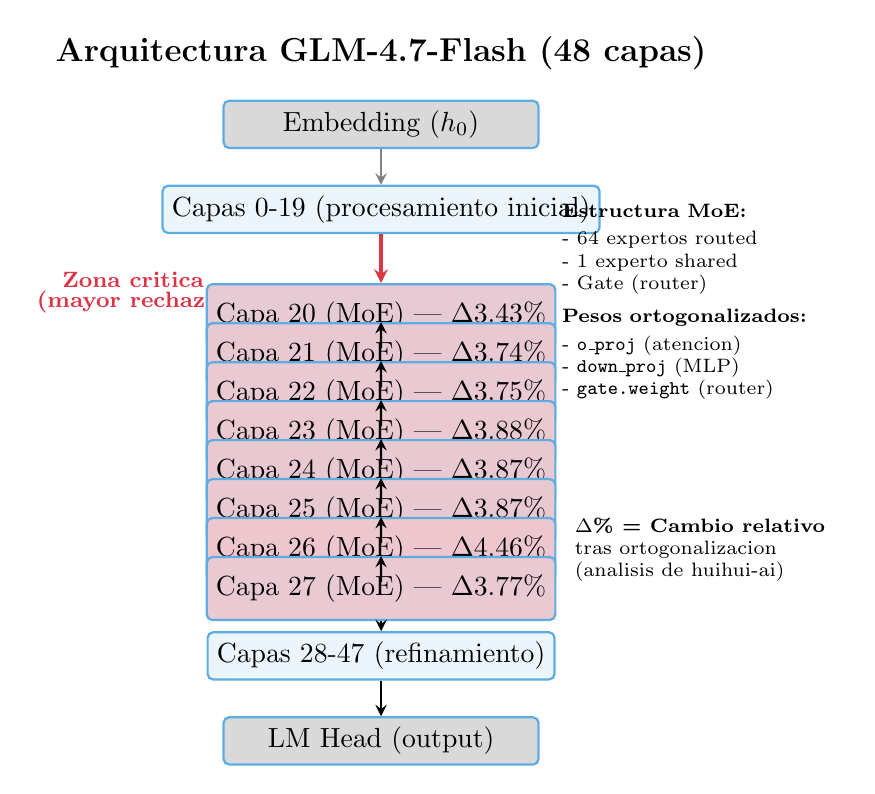
\begin{tikzpicture}[
    scale=0.9,
    layer/.style={draw=layer!80, fill=layer!20, thick, minimum width=4cm, minimum height=0.6cm, rounded corners=2pt},
    moe/.style={draw=layer!80, fill=layer!30, thick, minimum width=4cm, minimum height=0.8cm, rounded corners=2pt},
    arrow/.style={->, thick, >=stealth},
    label/.style={font=\footnotesize}
]

\node[font=\large\bfseries] at (2, 10.5) {Arquitectura GLM-4.7-Flash (48 capas)};
\node[layer, fill=gray!30] (embed) at (2, 9.5) {Embedding ($h_0$)};
\node[layer, fill=layer!10] (early) at (2, 8.3) {Capas 0-19 (procesamiento inicial)};
\draw[arrow, gray] (embed) -- (early);

\node[font=\footnotesize\bfseries, text=harmful] at (-1.5, 7.3) {Zona critica};
\node[font=\footnotesize\bfseries, text=harmful] at (-1.5, 7.0) {(mayor rechazo)};

\foreach \i/\change in {0/3.43, 1/3.74, 2/3.75, 3/3.88, 4/3.87, 5/3.87, 6/4.46, 7/3.77} {
    \pgfmathsetmacro{\y}{6.8 - \i*0.55}
    \pgfmathsetmacro{\layernum}{int(20 + \i)}
    \pgfmathsetmacro{\intensity}{20 + \change*15}
    \node[moe, fill=harmful!\intensity!layer!30] (layer\i) at (2, \y) {Capa \layernum\ (MoE) --- $\Delta$\change\%};
}

\draw[arrow, harmful, very thick] (early) -- (layer0);
\draw[arrow] (layer0) -- (layer1);
\draw[arrow] (layer1) -- (layer2);
\draw[arrow] (layer2) -- (layer3);
\draw[arrow] (layer3) -- (layer4);
\draw[arrow] (layer4) -- (layer5);
\draw[arrow] (layer5) -- (layer6);
\draw[arrow] (layer6) -- (layer7);

\node[layer, fill=layer!10] (late) at (2, 2.0) {Capas 28-47 (refinamiento)};
\draw[arrow] (layer7) -- (late);
\node[layer, fill=gray!30] (head) at (2, 0.8) {LM Head (output)};
\draw[arrow] (late) -- (head);

\node[align=left, font=\scriptsize, text width=3.5cm] at (6.5, 7) {
    \textbf{Estructura MoE:}\\[2pt]
    - 64 expertos routed\\
    - 1 experto shared\\
    - Gate (router)\\[4pt]
    \textbf{Pesos ortogonalizados:}\\[2pt]
    - \texttt{o\_proj} (atencion)\\
    - \texttt{down\_proj} (MLP)\\
    - \texttt{gate.weight} (router)
};

\node[align=left, font=\scriptsize] at (6.5, 3.5) {
    \textbf{$\Delta$\% = Cambio relativo}\\
    tras ortogonalizacion\\
    (analisis de huihui-ai)
};

\end{tikzpicture}

\newpage

% =============================================================================
% FIGURA 2: Espacio de activaciones y direccion de rechazo (pseudo-3D)
% =============================================================================
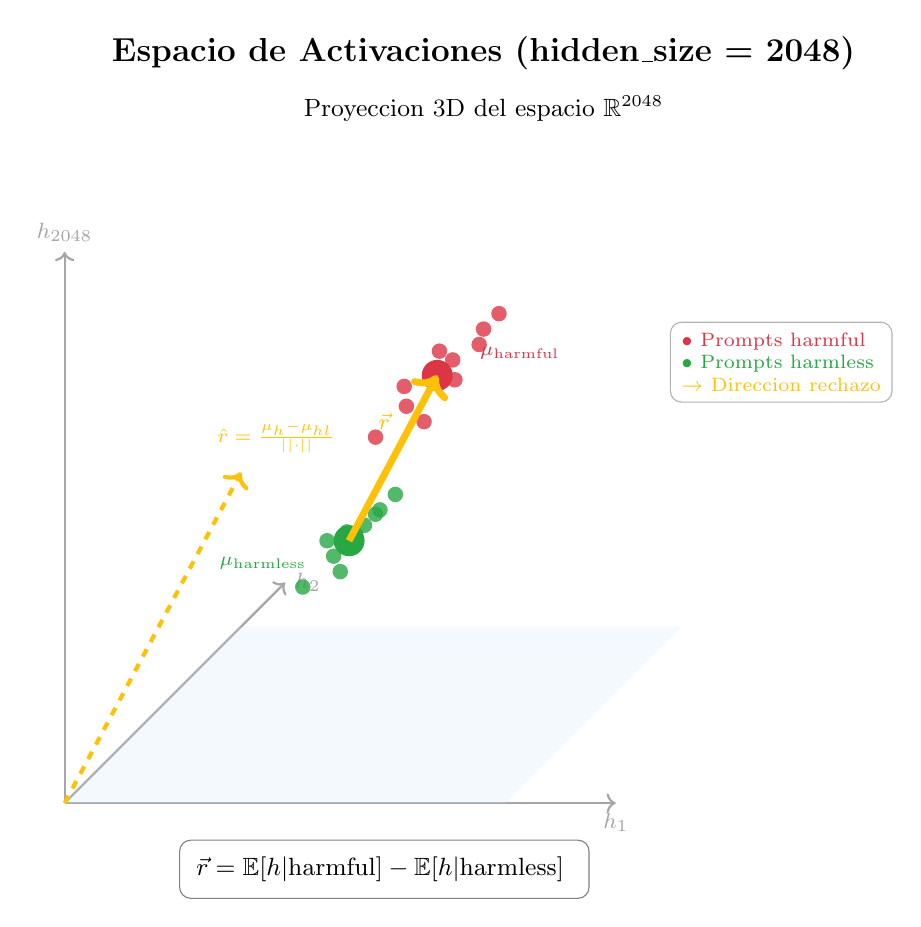
\begin{tikzpicture}[
    scale=1.4,
    x={(1cm,0cm)},
    y={(0.4cm,0.4cm)},
    z={(0cm,1cm)}
]

\node[font=\large\bfseries] at (3, 2, 6) {Espacio de Activaciones (hidden\_size = 2048)};
\node[font=\small] at (3, 2, 5.5) {Proyeccion 3D del espacio $\mathbb{R}^{2048}$};

% Ejes
\draw[->, thick, gray!70] (0,0,0) -- (5,0,0) node[anchor=north, font=\footnotesize]{$h_1$};
\draw[->, thick, gray!70] (0,0,0) -- (0,5,0) node[anchor=west, font=\footnotesize]{$h_2$};
\draw[->, thick, gray!70] (0,0,0) -- (0,0,5) node[anchor=south, font=\footnotesize]{$h_{2048}$};

% Plano base
\fill[layer!20, opacity=0.3] (0,0,0) -- (4,0,0) -- (4,4,0) -- (0,4,0) -- cycle;

% Nube de puntos harmful (rojo)
\foreach \x/\y/\z in {2.8/1.8/3.3, 2.5/1.5/3.0, 3.0/2.0/3.5, 2.7/1.4/2.9, 2.4/1.7/3.1,
                       3.1/2.1/3.6, 2.3/1.3/2.8, 2.9/1.6/3.2, 3.0/1.9/3.4, 2.6/2.0/3.3} {
    \fill[harmful, opacity=0.8] (\x, \y, \z) circle (2pt);
}

% Nube de puntos harmless (verde)
\foreach \x/\y/\z in {1.6/2.8/1.4, 1.4/2.6/1.2, 1.7/2.9/1.5, 1.5/2.5/1.1, 1.3/2.7/1.3,
                       1.8/3.0/1.6, 1.2/2.4/1.0, 1.6/2.6/1.4, 1.7/2.8/1.5, 1.4/2.9/1.3} {
    \fill[harmless, opacity=0.8] (\x, \y, \z) circle (2pt);
}

% Centroide harmful
\fill[harmful] (2.7, 1.7, 3.2) circle (4pt);
\node[font=\scriptsize, harmful, anchor=west] at (3.0, 1.7, 3.4) {$\mu_{\text{harmful}}$};

% Centroide harmless
\fill[harmless] (1.5, 2.7, 1.3) circle (4pt);
\node[font=\scriptsize, harmless, anchor=east] at (1.2, 2.7, 1.1) {$\mu_{\text{harmless}}$};

% Vector de rechazo
\draw[->, refusal, line width=2.5pt] (1.5, 2.7, 1.3) -- (2.7, 1.7, 3.2);
\node[font=\footnotesize, refusal, anchor=south] at (2.1, 2.0, 2.5) {$\vec{r}$};

% Direccion normalizada
\draw[->, refusal, line width=1.5pt, dashed] (0,0,0) -- (2.4, -2.0, 3.8);
\node[font=\scriptsize, refusal] at (2.8, -2.2, 4.2) {$\hat{r} = \frac{\mu_h - \mu_{hl}}{||\cdot||}$};

% Leyenda
\node[align=left, font=\scriptsize, draw=black!30, fill=white, rounded corners, inner sep=4pt] at (5.5, 2.5, 3) {
    \textcolor{harmful}{$\bullet$ Prompts harmful}\\
    \textcolor{harmless}{$\bullet$ Prompts harmless}\\
    \textcolor{refusal}{$\rightarrow$ Direccion rechazo}
};

% Formula
\node[align=center, font=\small, draw=black!50, rounded corners, fill=white, inner sep=6pt] at (2.5, 1, -1) {
    $\vec{r} = \mathbb{E}[h | \text{harmful}] - \mathbb{E}[h | \text{harmless}]$
};

\end{tikzpicture}

\newpage

% =============================================================================
% FIGURA 3: Ortogonalizacion de pesos (pseudo-3D)
% =============================================================================
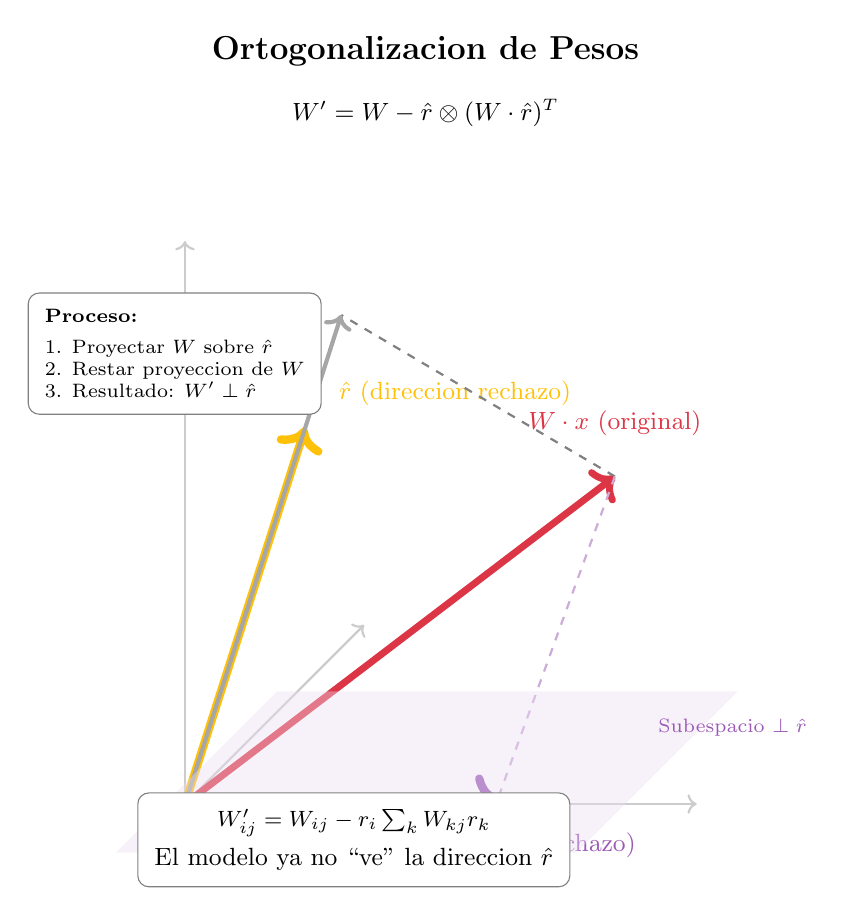
\begin{tikzpicture}[
    scale=1.3,
    x={(1cm,0cm)},
    y={(0.35cm,0.35cm)},
    z={(0cm,1cm)}
]

\node[font=\large\bfseries] at (2, 1, 7) {Ortogonalizacion de Pesos};
\node[font=\small] at (2, 1, 6.4) {$W' = W - \hat{r} \otimes (W \cdot \hat{r})^T$};

% Ejes sutiles
\draw[->, thick, gray!40] (0,0,0) -- (5,0,0);
\draw[->, thick, gray!40] (0,0,0) -- (0,5,0);
\draw[->, thick, gray!40] (0,0,0) -- (0,0,5.5);

% Direccion de rechazo
\draw[->, refusal, line width=3pt] (0,0,0) -- (1.0, 0.5, 3.5);
\node[font=\small, refusal, anchor=west] at (1.2, 0.6, 3.8) {$\hat{r}$ (direccion rechazo)};

% Vector original
\draw[->, harmful, line width=2.5pt] (0,0,0) -- (3.5, 2.0, 2.5);
\node[font=\small, harmful, anchor=south] at (3.5, 2.0, 2.8) {$W \cdot x$ (original)};

% Proyeccion
\draw[dashed, gray, thick] (3.5, 2.0, 2.5) -- (1.3, 0.65, 4.55);
\draw[->, gray!70, line width=1.5pt] (0,0,0) -- (1.3, 0.65, 4.55);
\node[font=\scriptsize, gray] at (0.5, 0.3, 4.8) {proyeccion};

% Vector ortogonalizado
\draw[->, orthogonal, line width=3pt] (0,0,0) -- (2.5, 1.6, -0.5);
\node[font=\small, orthogonal, anchor=north] at (2.7, 1.8, -0.8) {$W' \cdot x$ (sin rechazo)};

% Linea conectando
\draw[dashed, orthogonal!50, thick] (3.5, 2.0, 2.5) -- (2.5, 1.6, -0.5);

% Plano ortogonal
\fill[orthogonal!20, opacity=0.4] (-0.5,4,-0.3) -- (4,4,-0.3) -- (4,-0.5,-0.3) -- (-0.5,-0.5,-0.3) -- cycle;
\node[font=\scriptsize, orthogonal] at (4.3, 3, -0.3) {Subespacio $\perp \hat{r}$};

% Proceso
\node[align=left, font=\scriptsize, draw=black!50, rounded corners, fill=white, inner sep=6pt] at (-1.5, 4, 3) {
    \textbf{Proceso:}\\[3pt]
    1. Proyectar $W$ sobre $\hat{r}$\\
    2. Restar proyeccion de $W$\\
    3. Resultado: $W' \perp \hat{r}$
};

% Formula
\node[align=center, font=\footnotesize, draw=black!50, rounded corners, fill=white, inner sep=6pt] at (2, -1, 0) {
    $W'_{ij} = W_{ij} - r_i \sum_k W_{kj} r_k$\\[3pt]
    \small{El modelo ya no ``ve'' la direccion $\hat{r}$}
};

\end{tikzpicture}

\newpage

% =============================================================================
% FIGURA 4: Efecto antes/despues
% =============================================================================
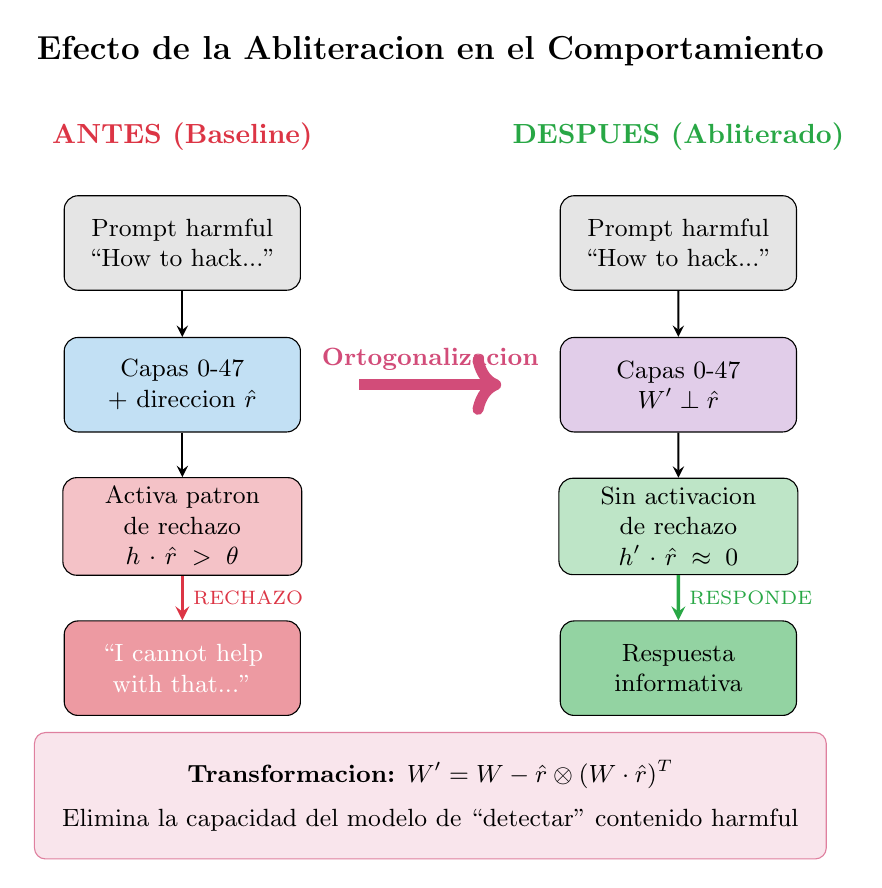
\begin{tikzpicture}[
    scale=0.9,
    box/.style={draw, rounded corners=5pt, minimum width=3cm, minimum height=1.2cm, align=center, font=\small},
    arrow/.style={->, thick, >=stealth}
]

\node[font=\large\bfseries] at (6, 9) {Efecto de la Abliteracion en el Comportamiento};

% ANTES
\node[font=\bfseries, harmful] at (2.5, 7.8) {ANTES (Baseline)};
\node[box, fill=gray!20] (in1) at (2.5, 6.3) {Prompt harmful\\``How to hack...''};
\node[box, fill=layer!30] (proc1) at (2.5, 4.3) {Capas 0-47\\+ direccion $\hat{r}$};
\node[box, fill=harmful!30, text width=2.8cm] (det1) at (2.5, 2.3) {Activa patron\\de rechazo\\$h \cdot \hat{r} > \theta$};
\node[box, fill=harmful!50, text=white] (out1) at (2.5, 0.3) {``I cannot help\\with that...''};

\draw[arrow] (in1) -- (proc1);
\draw[arrow] (proc1) -- (det1);
\draw[arrow, harmful, very thick] (det1) -- node[right, font=\scriptsize] {RECHAZO} (out1);

% DESPUES
\node[font=\bfseries, harmless] at (9.5, 7.8) {DESPUES (Abliterado)};
\node[box, fill=gray!20] (in2) at (9.5, 6.3) {Prompt harmful\\``How to hack...''};
\node[box, fill=orthogonal!30] (proc2) at (9.5, 4.3) {Capas 0-47\\$W' \perp \hat{r}$};
\node[box, fill=harmless!30, text width=2.8cm] (det2) at (9.5, 2.3) {Sin activacion\\de rechazo\\$h' \cdot \hat{r} \approx 0$};
\node[box, fill=harmless!50] (out2) at (9.5, 0.3) {Respuesta\\informativa};

\draw[arrow] (in2) -- (proc2);
\draw[arrow] (proc2) -- (det2);
\draw[arrow, harmless, very thick] (det2) -- node[right, font=\scriptsize] {RESPONDE} (out2);

% Flecha transformacion
\draw[->, line width=4pt, purple!70] (5, 4.3) -- node[above, font=\small\bfseries] {Ortogonalizacion} (7, 4.3);

% Ecuacion
\node[align=center, draw=purple!50, fill=purple!10, rounded corners, inner sep=10pt, font=\small] at (6, -1.5) {
    \textbf{Transformacion:} $W' = W - \hat{r} \otimes (W \cdot \hat{r})^T$\\[5pt]
    Elimina la capacidad del modelo de ``detectar'' contenido harmful
};

\end{tikzpicture}

\newpage

% =============================================================================
% FIGURA 5: Pipeline completo
% =============================================================================
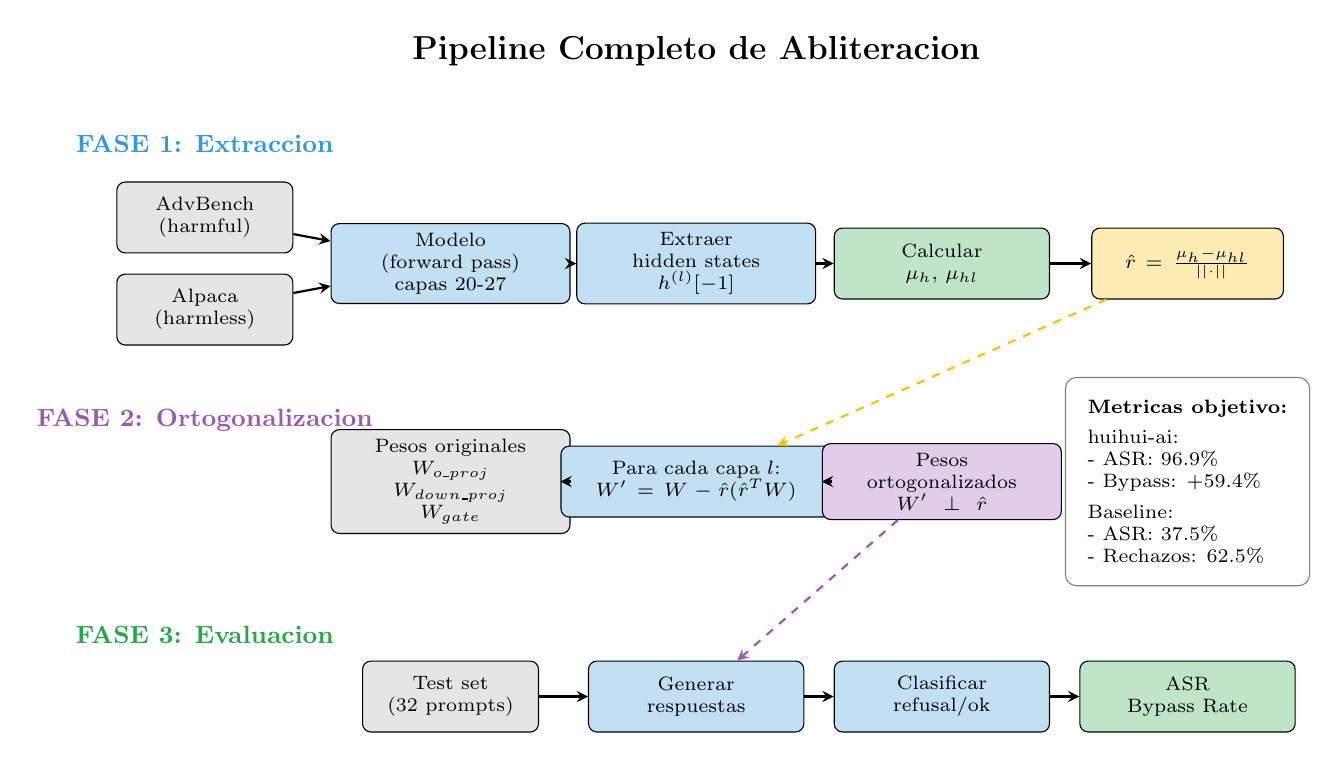
\begin{tikzpicture}[
    scale=0.78,
    block/.style={draw, rounded corners=3pt, minimum height=0.9cm, align=center, font=\scriptsize},
    data/.style={block, fill=gray!20},
    process/.style={block, fill=layer!30},
    result/.style={block, fill=harmless!30},
    arrow/.style={->, thick, >=stealth}
]

\node[font=\large\bfseries] at (8, 11.5) {Pipeline Completo de Abliteracion};

% FASE 1
\node[font=\small\bfseries, text=layer] at (0, 10) {FASE 1: Extraccion};
\node[data, text width=2cm] (adv) at (0, 8.8) {AdvBench\\(harmful)};
\node[data, text width=2cm] (alp) at (0, 7.3) {Alpaca\\(harmless)};
\node[process, text width=2.8cm] (model1) at (4, 8.05) {Modelo\\(forward pass)\\capas 20-27};
\node[process, text width=2.8cm] (extract) at (8, 8.05) {Extraer\\hidden states\\$h^{(l)}[-1]$};
\node[result, text width=2.5cm] (means) at (12, 8.05) {Calcular\\$\mu_h$, $\mu_{hl}$};
\node[result, text width=2.2cm, fill=refusal!30] (refdir) at (16, 8.05) {$\hat{r} = \frac{\mu_h - \mu_{hl}}{||\cdot||}$};

\draw[arrow] (adv) -- (model1);
\draw[arrow] (alp) -- (model1);
\draw[arrow] (model1) -- (extract);
\draw[arrow] (extract) -- (means);
\draw[arrow] (means) -- (refdir);

% FASE 2
\node[font=\small\bfseries, text=orthogonal] at (0, 5.5) {FASE 2: Ortogonalizacion};
\node[data, text width=2.8cm] (weights) at (4, 4.5) {Pesos originales\\$W_{o\_proj}$\\$W_{down\_proj}$\\$W_{gate}$};
\node[process, text width=3.2cm] (ortho) at (8, 4.5) {Para cada capa $l$:\\$W' = W - \hat{r}(\hat{r}^T W)$};
\node[result, text width=2.8cm, fill=orthogonal!30] (newweights) at (12, 4.5) {Pesos\\ortogonalizados\\$W' \perp \hat{r}$};

\draw[arrow] (weights) -- (ortho);
\draw[arrow, refusal, dashed, thick] (refdir) -- (ortho);
\draw[arrow] (ortho) -- (newweights);

% FASE 3
\node[font=\small\bfseries, text=harmless] at (0, 2) {FASE 3: Evaluacion};
\node[data, text width=2cm] (test) at (4, 1) {Test set\\(32 prompts)};
\node[process, text width=2.5cm] (gen) at (8, 1) {Generar\\respuestas};
\node[process, text width=2.5cm] (classify) at (12, 1) {Clasificar\\refusal/ok};
\node[result, text width=2.5cm] (metrics) at (16, 1) {ASR\\Bypass Rate};

\draw[arrow] (test) -- (gen);
\draw[arrow, orthogonal, dashed, thick] (newweights) -- (gen);
\draw[arrow] (gen) -- (classify);
\draw[arrow] (classify) -- (metrics);

% Metricas
\node[align=left, draw=black!50, rounded corners, fill=white, inner sep=8pt, font=\scriptsize] at (16, 4.5) {
    \textbf{Metricas objetivo:}\\[3pt]
    huihui-ai:\\
    - ASR: 96.9\%\\
    - Bypass: +59.4\%\\[3pt]
    Baseline:\\
    - ASR: 37.5\%\\
    - Rechazos: 62.5\%
};

\end{tikzpicture}

\newpage

% =============================================================================
% FIGURA 6: Estrategias
% =============================================================================
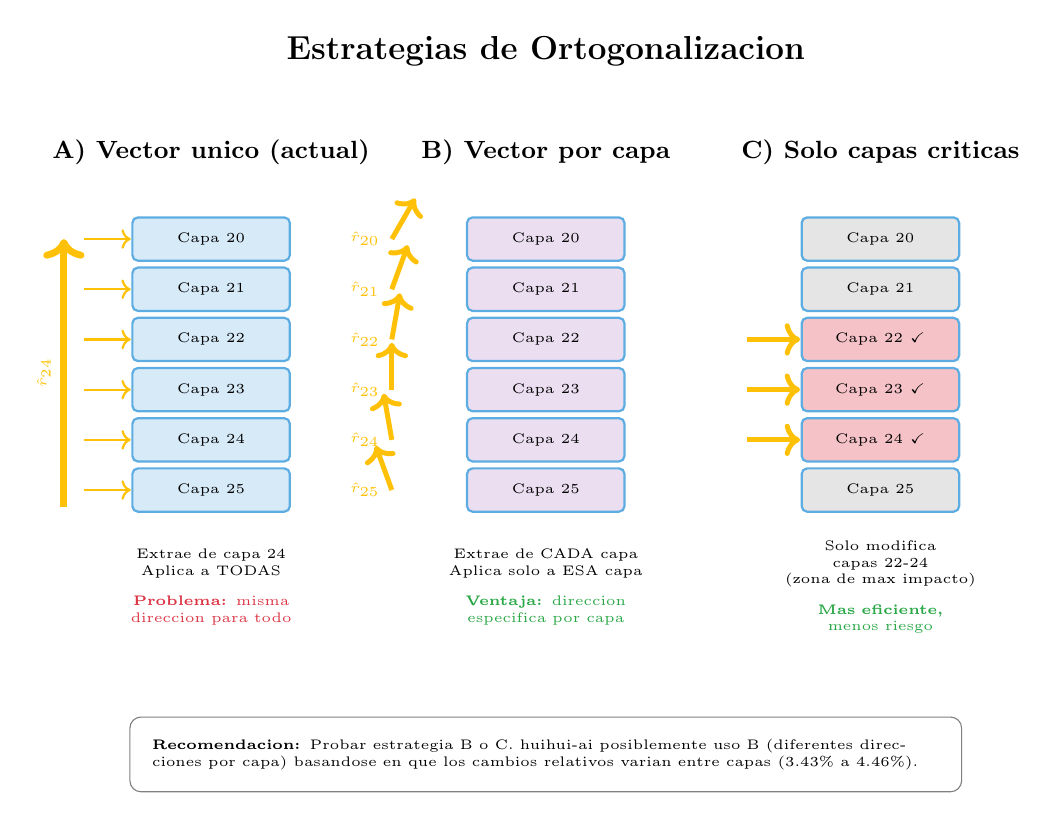
\begin{tikzpicture}[
    scale=0.85,
    layer/.style={draw=layer!80, fill=layer!20, thick, minimum width=2cm, minimum height=0.55cm, rounded corners=2pt, font=\tiny},
    arrow/.style={->, thick, >=stealth}
]

\node[font=\large\bfseries] at (7.5, 10) {Estrategias de Ortogonalizacion};

% A) Vector unico
\node[font=\small\bfseries] at (2.5, 8.5) {A) Vector unico (actual)};
\foreach \i in {0,...,5} {
    \pgfmathsetmacro{\y}{7.2 - \i*0.75}
    \pgfmathsetmacro{\layernum}{int(20 + \i)}
    \node[layer] (a\i) at (2.5, \y) {Capa \layernum};
}
\draw[->, refusal, line width=2.5pt] (0.3, 3.2) -- (0.3, 7.2);
\node[font=\tiny, refusal, rotate=90] at (0, 5.2) {$\hat{r}_{24}$};
\foreach \i in {0,...,5} {
    \pgfmathsetmacro{\y}{7.2 - \i*0.75}
    \draw[->, refusal, thick] (0.6, \y) -- (1.3, \y);
}
\node[align=center, font=\tiny, text width=2.5cm] at (2.5, 2) {
    Extrae de capa 24\\
    Aplica a TODAS\\[5pt]
    \textcolor{harmful}{\textbf{Problema:} misma}\\
    \textcolor{harmful}{direccion para todo}
};

% B) Vector por capa
\node[font=\small\bfseries] at (7.5, 8.5) {B) Vector por capa};
\foreach \i in {0,...,5} {
    \pgfmathsetmacro{\y}{7.2 - \i*0.75}
    \pgfmathsetmacro{\layernum}{int(20 + \i)}
    \node[layer, fill=orthogonal!20] (b\i) at (7.5, \y) {Capa \layernum};
}
\foreach \i in {0,...,5} {
    \pgfmathsetmacro{\y}{7.2 - \i*0.75}
    \pgfmathsetmacro{\angle}{60 + \i*10}
    \pgfmathsetmacro{\layernum}{int(20 + \i)}
    \draw[->, refusal, line width=1.8pt] (5.2, \y) -- ++(\angle:0.7);
    \node[font=\tiny, refusal] at (4.8, \y) {$\hat{r}_{\layernum}$};
}
\node[align=center, font=\tiny, text width=2.8cm] at (7.5, 2) {
    Extrae de CADA capa\\
    Aplica solo a ESA capa\\[5pt]
    \textcolor{harmless}{\textbf{Ventaja:} direccion}\\
    \textcolor{harmless}{especifica por capa}
};

% C) Solo criticas
\node[font=\small\bfseries] at (12.5, 8.5) {C) Solo capas criticas};
\foreach \i in {0,...,5} {
    \pgfmathsetmacro{\y}{7.2 - \i*0.75}
    \pgfmathsetmacro{\layernum}{int(20 + \i)}
    \ifnum\i>1
        \ifnum\i<5
            \node[layer, fill=harmful!30] (c\i) at (12.5, \y) {Capa \layernum\ $\checkmark$};
            \draw[->, refusal, line width=1.8pt] (10.5, \y) -- (11.3, \y);
        \else
            \node[layer, fill=gray!20] (c\i) at (12.5, \y) {Capa \layernum};
        \fi
    \else
        \node[layer, fill=gray!20] (c\i) at (12.5, \y) {Capa \layernum};
    \fi
}
\node[align=center, font=\tiny, text width=2.8cm] at (12.5, 2) {
    Solo modifica\\
    capas 22-24\\
    (zona de max impacto)\\[5pt]
    \textcolor{harmless}{\textbf{Mas eficiente,}}\\
    \textcolor{harmless}{menos riesgo}
};

% Recomendacion
\node[draw=black!50, rounded corners, fill=white, inner sep=8pt, font=\tiny, text width=10cm, align=left] at (7.5, -0.5) {
    \textbf{Recomendacion:} Probar estrategia B o C. huihui-ai posiblemente uso B (diferentes direcciones por capa) basandose en que los cambios relativos varian entre capas (3.43\% a 4.46\%).
};

\end{tikzpicture}

\end{document}
